In this chapter I analyse the data that have been extracted by eth2dgraph. Each section describes an independent analysis.

All the results refer to data from block $0$ to block $17,265,420$ of the Ethereum mainnet. It corresponds to the period of time between July 30 2015 to May 15 2023 (7 years, 9 months and 15 days).

\section{General data overview}

This analysis wants to give a general overview of the data extracted. There are some interesting numbers that help to understand the current state of the Ethereum chain. Here are some interesting points:

\begin{itemize}
    \item 60,016,663 smart contract deployments were found with 59,429,189 unique addresses. 88\% of them (52,343,783) never emitted logs. 87\% of them (51,974,197) never received a single transaction. Just 5.78\% (3,435,332) of contracts' addresses both received at least a transaction and emitted at least one log. This shows that the majority of the deployed smart contracts are never used.
    
    \item There are 2.8M logs emitted. 10 smart contracts alone, reported in \cref{table:top-logs-emitters}, emitted the 24.25\% of all logs. Top 100 contracts emitted 38.83\% of the logs. Top 1,000 contracts emitted 57.53\% of the logs. 33,287 smart contracts (0.056\% of the total) emitted 90\% of the logs. Most of the activity on the chain is restricted to a relatively small group of smart contracts.
    
    \item Transactions are more evenly distributed. There are 165,684,328 distinct EOAs that have sent transactions. Top 10 senders sent 6.96\% of all transactions. 90\% of transactions were sent by top 25\% addresses. 
    
    \item There are 286,391,265 distinct addresses that have received transactions. Top 10 receivers received 18.55\% of all the transactions, there is just one receiver in the top 10 that is not a contract\footnote{It is an address of the Coinbase exchange {\tt 0xa090e606e30bd747d4e6245a1517ebe430f0057e}.}. 90\% of transactions were received by top 57.85\% receivers.
    
    \item 61.92\% of transactions are sent to smart contracts. 0.25\% are sent to the null address {\tt 0x0}. The remaining 37.83\% are transactions from EOAs to other EOAs or unclaimed addresses.
    
    \item \cref{fig:deploy-history} shows the history of smart contracts deployments. The growth in deployments was exponential until the beginning of 2018. After an initial period in which there were more deployments done by users than by contracts, now the majority of smart contracts are deployed using the CREATE or CREATE2 opcodes. This confirms the trend observed by Kiffer et al.~\cite{ethereum-sc-topology}. They observed this phenomena in data until 2018. The difference in deployments by users or by contracts has grown since then. Since 2019, the difference is of at least one order of magnitude.
\end{itemize}

\begin{table}[H]
\centering
    \begin{threeparttable}
    \begin{tabular}{ c c c } 
    \toprule
    \textbf{Name of contract} & \textbf{Contract address} & \textbf{Logs emitted} \\
    \midrule
       Wrapped Ether & \small{0xc02aaa39b223fe8d0a0e5c4f27ead9083c756cc2} & 282,095,104  \\ [1.2ex]
       Tether USD  & \small{0xdac17f958d2ee523a2206206994597c13d831ec7} & 196,788,993  \\ [1.2ex]
       USD Coin & \small{0xa0b86991c6218b36c1d19d4a2e9eb0ce3606eb48} & 74,321,927  \\ [1.2ex]
       XEN & \small{0x06450dee7fd2fb8e39061434babcfc05599a6fb8} & 30,438,737  \\ [1.2ex]
       DAI Stablecoin& \small{0x6b175474e89094c44da98b954eedeac495271d0f} & 20,283,129  \\ [1.2ex]
       Seaport & \small{0x00000000006c3852cbef3e08e8df289169ede581} & 16,764,010  \\ [1.2ex]
       ChainLink Token & \small{0x514910771af9ca656af840dff83e8264ecf986ca} & 16,698,857  \\ [1.2ex]
       Wyvern Exchange & \small{0x7be8076f4ea4a4ad08075c2508e481d6c946d12b} & 15,735,740  \\ [1.2ex]
       SHIBA INU & \small{0x95ad61b0a150d79219dcf64e1e6cc01f0b64c4ce} & 12,607,046  \\ [1.2ex]
       Forsage & \small{0x5acc84a3e955bdd76467d3348077d003f00ffb97} & 12,323,018  \\ [1.2ex]  
    \bottomrule
    \end{tabular}
    \end{threeparttable}
    \caption{Top 10 smart contracts per logs emitted.}
    \label{table:top-logs-emitters}
\end{table}

\begin{figure}[H]
    \centering
    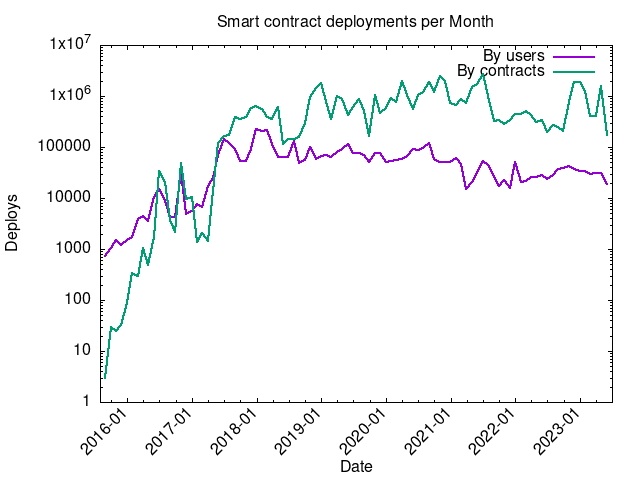
\includegraphics[width=0.9\textwidth]{Figures/analysis/deploys_per_month.png}
    \caption{Smart contract deployments over time grouped by month.}
    \label{fig:deploy-history}
\end{figure}

\section{Skeleton clusters}

The skeleton of a smart contract is its deployed bytecode without the arguments of the PUSH opcodes and the eventual metadata appended at the end. \cref{skeleton-section} describes this concept in details and explains how eth2dgraph extracts the skeletons from the Ethereum chain.

Out of the 60M smart contracts deployments in the history of Ethereum, just 467K distinct skeletons were found. This allows to link smart contracts with each other based on skeleton equality. On average, each smart contract has 128 semantically identical siblings. 

The distribution of smart contracts by skeleton is not uniform. There are 361,546 skeletons (77.4\%) that correspond to a single deployed Ethereum smart contract. At the same time there are skeletons that correspond to millions of smart contract deployments. The most frequently used skeleton matched 12.2M deployments.

\subsection{Most deployed skeletons}

I here analyze the top 10 skeletons found on the Ethereum chain by number of deployments. These 10 distinct skeleton corresponds together to 44,389,576 smart contract deployments (73.96\% of the total).

\begin{itemize}

    \item The most used skeleton is related to gas reserves. It is the way gas tokens store gas when it is bought. The concept of gas token is analyzed in \cref{gas-tokens}. This skeleton has a very simple bytecode that just allows a particular address, with length of 14 bytes, to destroy the contract. The size of this skeleton is of 21 bytes. It has been deployed 12,240,689 times.
    
    \item The second skeleton is the implementation of the ERC-1167\footnote{Specification of the ERC-1167 Minimal Proxy Contract: \url{https://eips.ethereum.org/EIPS/eip-1167}} logic. This bytecode consists in a minimal proxy that forwards all the calls it receives to a fixed hard-coded address. The size of this skeleton is of 45 bytes. It has been used 11,168,872 times.

    \item The third skeleton is again related to gas tokens. It is the same logic of the first described skeleton, but with the allowed address of 15 bytes instead of 14. It has been used 6,829,142 times. Its size is of 22 bytes.

    \item The fourth skeleton is simply the empty bytecode. It is valid in the Ethereum protocol to have empty smart contracts. 4,877,139 deployments with no bytecode were found.

    \item The fifth skeleton is again related to gas tokens. It is the same logic of the previous two but with the length of allowed address of 20 bytes. 2,138,723 deployments matching this skeleton were found.

    \item The sixth skeleton represents 1,665,668 user wallets of the \textit{Bittrex} exchange\footnote{Bittrex is a crypto exchange platform: \url{https://global.bittrex.com/}.}. Each of these smart contract is a controlled wallet. This means that each contract represents a user of the exchange, but the control over the Ethers and tokens remains under the company. The point of having these controlled wallets is to give users a unique address to send their tokens or Ethers. The size of this skeleton is of 502 bytes.

    \item The seventh skeleton has been used 1,549,146 times and represents an \textit{OwnableDelegateProxy}. It is a proxy contract, so it simply forwards the received calls to another contract that implements the actual logic, using {\tt delegatecall}. This specific type of proxy has two additional properties:
    \begin{itemize}
        \item \textit{Ownable}: it stores the address of the owner and allows it to modify the implementation address. The ownership can eventually be transferred.
        \item \textit{Upgradable}: it is possible to update the address of the implementation, changing where the proxy is forwarding the calls.
    \end{itemize}
    All the previous logic is implemented in a bytecode with a size of 1073 bytes.

    \item The eighth skeleton has been used 1,542,310 times and represents a \textit{forwarder contract}. This skeleton has two main public functions: \textit{flush()} and \textit{flushTokens(address)}. They are used to transfer respectively ETH and tokens to a fixed parent address. The point of this kind of contract is to have multiple receive address for the same wallet. ETH transfers are automatically sent to the parent address, while tokens can be flushed with a transaction. Bitgo\footnote{Bitgo is a digital asset trust company: \url{https://www.bitgo.com/}} uses this contract in their implementation of the multisignature wallet\footnote{Source code of the multisignature wallet: \url{https://github.com/BitGo/eth-multisig-v2/tree/master}}. The size of this skeleton is of 785 bytes.

    \item The nineth skeleton is a proxy used for the Ambi Multisig wallet~\cite{wallet-contracts}. It has been deployed 1,202,291 times. 

    \item The tenth skeleton has been used 1,175,596 times and it is the exact same forwarding logic of the eight skeleton. The few small differences are probably due to compiler version or optimization level. Its size is of 789 bytes.
    
\end{itemize}

I calculated cosine and interface similarity of the top 10 skeletons to find similarities between them and all the other skeletons. This formed seven clusters shown in \cref{table:top-skeletons-clusters}.

These 7 clusters describe 75.29\% of all the deployments that happened in the Ethereum blockchain. They can be grouped in just 4 distinct categories: \textit{gas token}, \textit{proxy}, \textit{wallet} and \textit{empty contract}.

\begin{table}[H]
\centering
    \begin{threeparttable}
    \begin{tabular}{ c c c c } 
    \toprule
    \textbf{\# Group} & \textbf{Distinct skeletons} & \textbf{Deployments} & \textbf{Category} \\
    \midrule  
    1 & 5 & 21,787,384 & Gas token \\ [1.2ex]
    2 & 6 & 11,169,089 & Proxy \\ [1.2ex]
    3 & 1 & 4,877,139 & Empty contract \\ [1.2ex]
    4 & 31 & 2,732,644 & Wallet \\ [1.2ex]
    5 & 5 & 1,863,898 & Wallet \\ [1.2ex]
    6 & 20 & 1,55,2654 & Proxy \\ [1.2ex]
    7 & 3 & 1,202,787 & Wallet \\ [1.2ex]
    \bottomrule
    \end{tabular}
    \end{threeparttable}
    \caption{Clusters formed by grouping top 10 skeletons with their similars.}
    \label{table:top-skeletons-clusters}
\end{table}

\subsection{New skeletons over time}

An interesting metric to observe is when the skeletons were first seen on the blockchain. This is a different indicator to the one shown in \cref{fig:deploy-history}, since it just shows when semantically new smart contracts are deployed, avoiding all the replicas.

\cref{fig:skeletons-deploy} shows, for each month, the amount of new skeletons found on the Ethereum chain. While the number of monthly deployments has not increased since 2021, the number of new monthly skeletons has kept increasing. This is also visible in \cref{fig:skeletons-ratio}, especially in the year of 2022 in which the ratio between deployments and new skeleton was low compared to the past. From this data, it appears that code reuse is dropping. 

\begin{figure}[H]
    \centering
    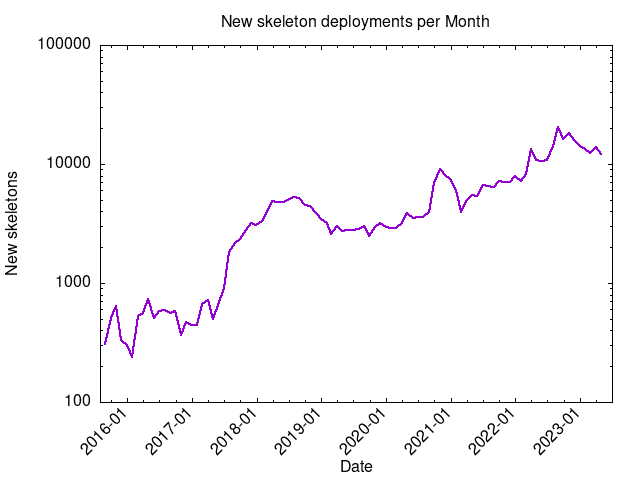
\includegraphics[width=0.9\textwidth]{Figures/analysis/skeletons_per_month.png}
    \caption{Deployments of new skeletons over time, grouped by month}
    \label{fig:skeletons-deploy}
\end{figure}

\begin{figure}[H]
    \centering
    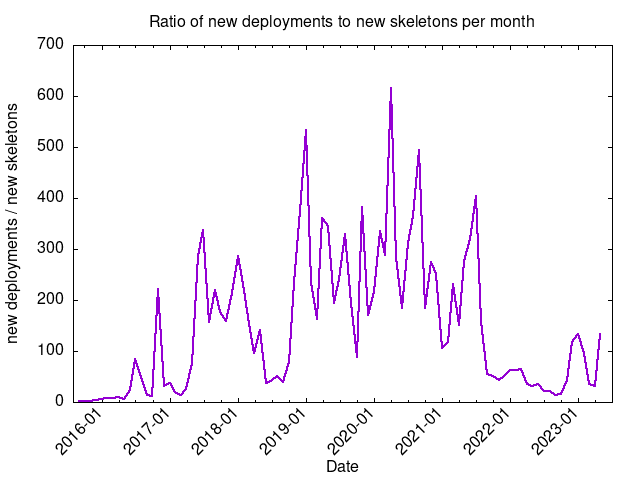
\includegraphics[width=0.9\textwidth]{Figures/analysis/ratio_per_month.png}
    \caption{Ratio of deployments to new skeletons over time, grouped by month. High values = more duplicates deployed.}
    \label{fig:skeletons-ratio}
\end{figure}

\section{Most used functions and events}

To give a 

\section{Token contracts}

The most common usage of smart contracts are tokens. There are two important standards that defined how token contracts must behave: ERC20 and ERC721. It is not possible to easily recognize them whit just the deployed bytecode stored on the blockchain. Here, I propose and verify some metrics to recognize them.

\section{Metamorphic contracts}

- explain how metamorphic contracts work
- 

\section{Gas tokens}
\label{gas-tokens}

The aim of this analysis is to study the impact of the \textit{GasToken} pattern on Ethereum.

GasToken is a pattern that was heavily used on the Ethereum blockchain to save on gas fees. It exploited the concept of refund provided by the opcodes {\tt SELFDESTRUCT} or {\tt SSTORE}. 
I here analyze the pattern that uses {\tt SELFDESTRUCT}. It works by creating and destroying very basic smart contracts, used as gas reserves. 

This pattern caused the creation of many fuzzy contracts and state slots that increased the size of the Ethereum state for useless motivations. It was the main reason for the adoption of EIP-3529~\cite{eip-3529}, that removed refunds for {\tt SELFDESTRUCT} and reduced {\tt SSTORE} refunds, effectively killing this pattern. This EIP was introduced on August 5th, 2021. It successfully killed the gas tokens as shown from the data I have observed.

The following information explains how this patter worked before EIP-3529. These two concepts are the fundamentals of this pattern: 

\begin{itemize}
    \item When a contract is deployed, the creator needs to pay $32000$ gas + $200$ gas for each non-zero byte stored.

    \item When a contract is destroyed, a refund of $24000$ gas is provided to the destroyer, after paying $700$ + $5000$ gas for calling {\tt CALL} + {\tt SELFDESTRUCT}. 
\end{itemize}

So the idea is that users deploy fuzzy contracts when gas is cheap and destroy them when gas is expensive. Gas from the refunds can cover up to 50\% of the gas used by the calling transaction that triggered the destructions, this is a cap introduced by the Ethereum protocol. 

To make this concept accessible, there are a few smart contracts that abstract the logic into simple tokens. For each token minted, there is an underlying smart contract deployment. This token can easily be transferred between users. When the token is freed, the underlying smart contract is destroyed and the destroyer gets a discount on the gas of the transaction. The two most used tokens are CHI\footnote{Chi Gastoken on Etherscan: \url{https://etherscan.io/token/0x0000000000004946c0e9F43F4Dee607b0eF1fA1c}} and GST2\footnote{GST2 token on Etherscan: \url{https://etherscan.io/token/0x0000000000b3F879cb30FE243b4Dfee438691c04}}.

To be profitable, the price of the gas when tokens are bought must be at least half of the price of the gas when they are sold. 

Gas price has been historically very volatile, so the existence of this pattern makes sense. \cref{fig:gas-price} shows the historical fluctuation of gas price.

\begin{figure}[H]
    \centering
    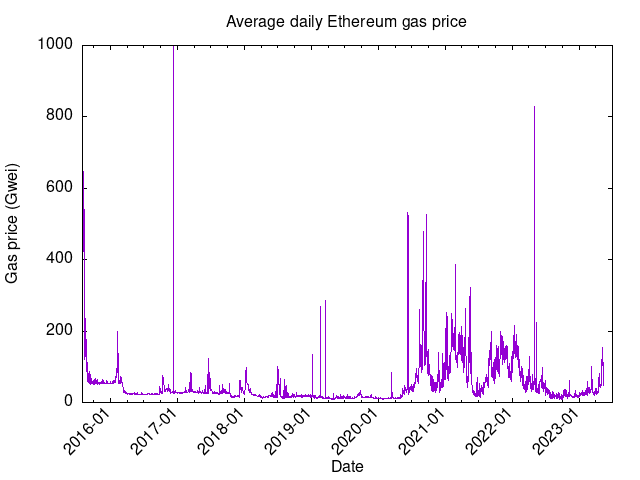
\includegraphics[width=0.9\textwidth]{Figures/analysis/gas-price.png}
    \caption{Average daily Ethereum gas price over time.}
    \label{fig:gas-price}
\end{figure}

\subsection{Identification of gas reserves}

I identified all the smart contract deployments that were used as gas reserves. The logic of a gas reserve contract is basic. It simply allows one hard-coded address to destruct it. \cref{lst:gas-token-code} shows the code that implements this logic, it is translated to the EVM bytecode reported in \cref{lst:gas-token-bytecode}

\begin{lstlisting}[caption={Pseudo code of the gas reserves.},label={lst:gas-token-code},captionpos=b,numbers=none]
if (msg.sender == GAS_TOKEN_ADDRESS) {
    SELFDESTRUCT(msg.sender);
}
\end{lstlisting}

\begin{lstlisting}[caption={EVM bytecode of the gas reserves.},label={lst:gas-token-bytecode},captionpos=b,numbers=none]
PUSH* <address of token contract>
CALLER
XOR
PC
JUMPI
CALLER
SELFDESTRUCT
\end{lstlisting}

The {\tt PUSH} opcode is represented as {\ *} because there are different implementations. Here it is possible to perform optimisations. The shortest the owner’s address is and the less bytes are needed to be stored in the contract storage. This results in cheaper deploys and more efficiency of the pattern.

For example, the GST2 gastoken has this address: {\tt 0xb3f879cb30fe243b4dfee438691c04} that are 15 bytes. The CHI gas token, a more recent and optimized alternative, uses {\tt 0x4946c0e9f43f4dee607b0ef1fa1c} that is one less byte. Finding these short addresses is a very resource-intensive computation and requires trillions of iterations and hashes.


\section{Contracts metadata}

- say which metadata have been extracted
- show data of metadata


\section{Contract creators}

- 
